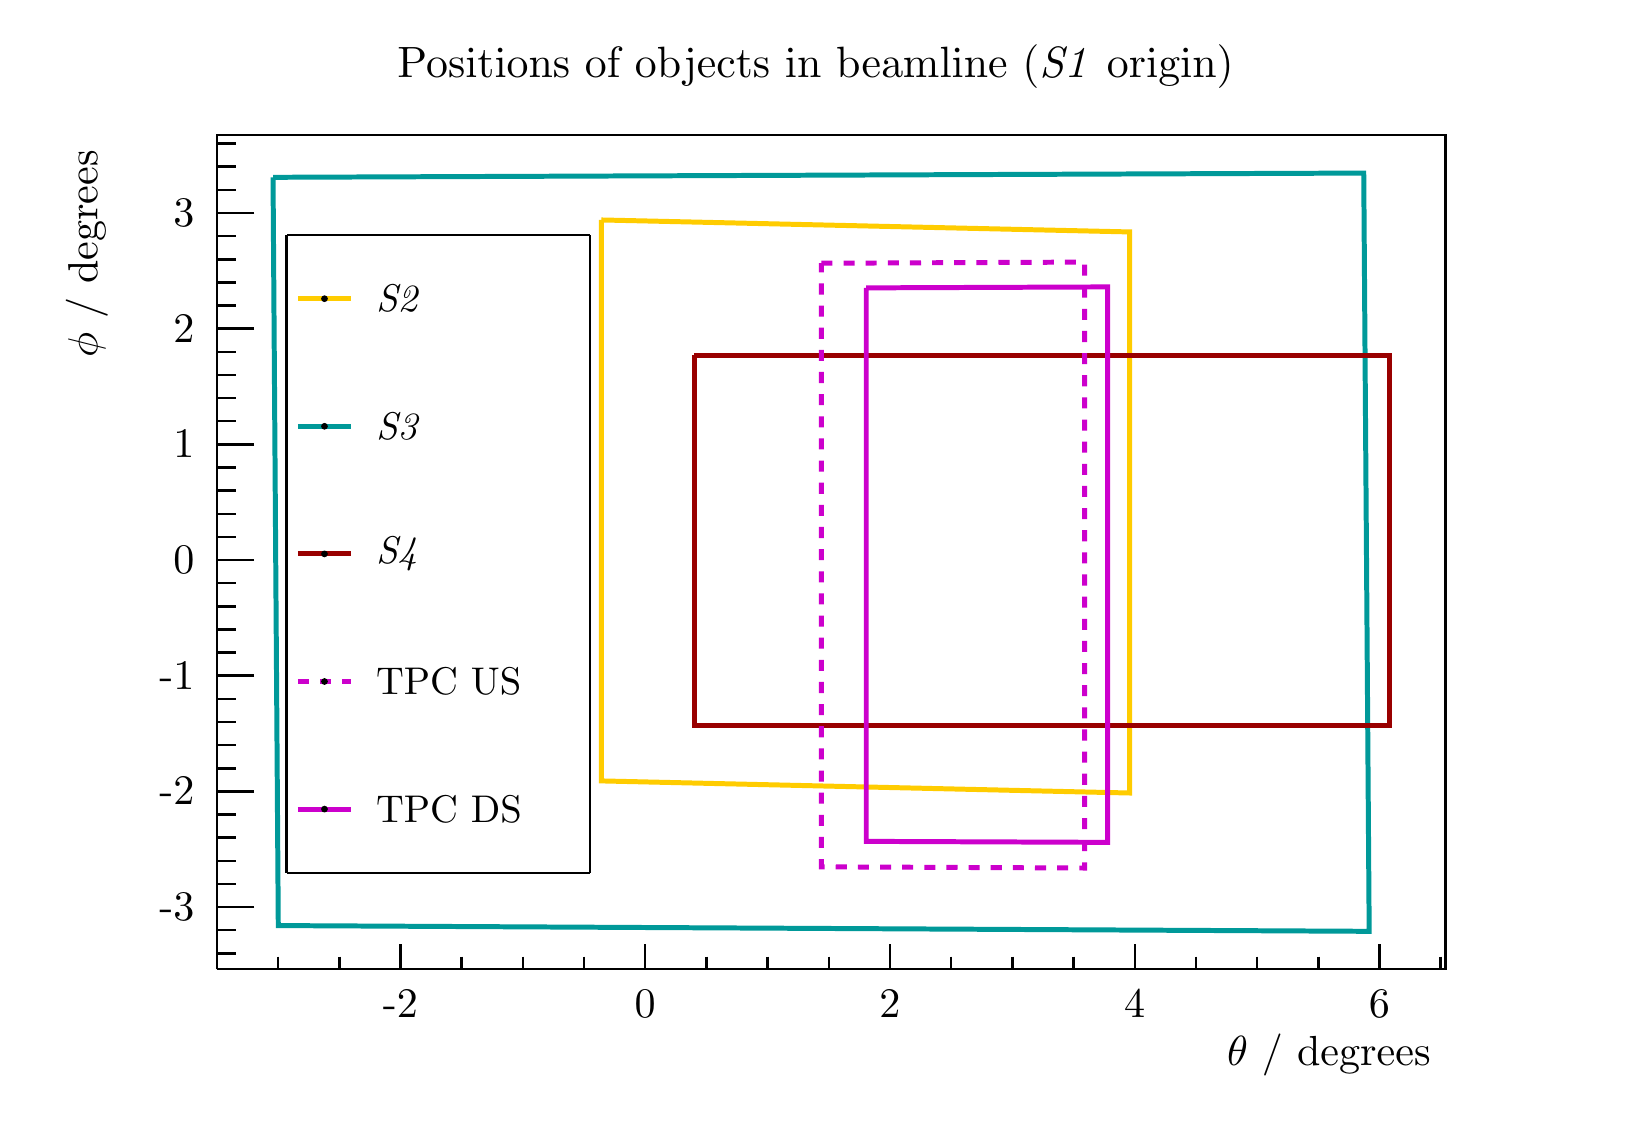
\begin{tikzpicture}
\pgfdeclareplotmark{cross} {
\pgfpathmoveto{\pgfpoint{-0.3\pgfplotmarksize}{\pgfplotmarksize}}
\pgfpathlineto{\pgfpoint{+0.3\pgfplotmarksize}{\pgfplotmarksize}}
\pgfpathlineto{\pgfpoint{+0.3\pgfplotmarksize}{0.3\pgfplotmarksize}}
\pgfpathlineto{\pgfpoint{+1\pgfplotmarksize}{0.3\pgfplotmarksize}}
\pgfpathlineto{\pgfpoint{+1\pgfplotmarksize}{-0.3\pgfplotmarksize}}
\pgfpathlineto{\pgfpoint{+0.3\pgfplotmarksize}{-0.3\pgfplotmarksize}}
\pgfpathlineto{\pgfpoint{+0.3\pgfplotmarksize}{-1.\pgfplotmarksize}}
\pgfpathlineto{\pgfpoint{-0.3\pgfplotmarksize}{-1.\pgfplotmarksize}}
\pgfpathlineto{\pgfpoint{-0.3\pgfplotmarksize}{-0.3\pgfplotmarksize}}
\pgfpathlineto{\pgfpoint{-1.\pgfplotmarksize}{-0.3\pgfplotmarksize}}
\pgfpathlineto{\pgfpoint{-1.\pgfplotmarksize}{0.3\pgfplotmarksize}}
\pgfpathlineto{\pgfpoint{-0.3\pgfplotmarksize}{0.3\pgfplotmarksize}}
\pgfpathclose
\pgfusepathqstroke
}
\pgfdeclareplotmark{cross*} {
\pgfpathmoveto{\pgfpoint{-0.3\pgfplotmarksize}{\pgfplotmarksize}}
\pgfpathlineto{\pgfpoint{+0.3\pgfplotmarksize}{\pgfplotmarksize}}
\pgfpathlineto{\pgfpoint{+0.3\pgfplotmarksize}{0.3\pgfplotmarksize}}
\pgfpathlineto{\pgfpoint{+1\pgfplotmarksize}{0.3\pgfplotmarksize}}
\pgfpathlineto{\pgfpoint{+1\pgfplotmarksize}{-0.3\pgfplotmarksize}}
\pgfpathlineto{\pgfpoint{+0.3\pgfplotmarksize}{-0.3\pgfplotmarksize}}
\pgfpathlineto{\pgfpoint{+0.3\pgfplotmarksize}{-1.\pgfplotmarksize}}
\pgfpathlineto{\pgfpoint{-0.3\pgfplotmarksize}{-1.\pgfplotmarksize}}
\pgfpathlineto{\pgfpoint{-0.3\pgfplotmarksize}{-0.3\pgfplotmarksize}}
\pgfpathlineto{\pgfpoint{-1.\pgfplotmarksize}{-0.3\pgfplotmarksize}}
\pgfpathlineto{\pgfpoint{-1.\pgfplotmarksize}{0.3\pgfplotmarksize}}
\pgfpathlineto{\pgfpoint{-0.3\pgfplotmarksize}{0.3\pgfplotmarksize}}
\pgfpathclose
\pgfusepathqfillstroke
}
\pgfdeclareplotmark{newstar} {
\pgfpathmoveto{\pgfqpoint{0pt}{\pgfplotmarksize}}
\pgfpathlineto{\pgfqpointpolar{44}{0.5\pgfplotmarksize}}
\pgfpathlineto{\pgfqpointpolar{18}{\pgfplotmarksize}}
\pgfpathlineto{\pgfqpointpolar{-20}{0.5\pgfplotmarksize}}
\pgfpathlineto{\pgfqpointpolar{-54}{\pgfplotmarksize}}
\pgfpathlineto{\pgfqpointpolar{-90}{0.5\pgfplotmarksize}}
\pgfpathlineto{\pgfqpointpolar{234}{\pgfplotmarksize}}
\pgfpathlineto{\pgfqpointpolar{198}{0.5\pgfplotmarksize}}
\pgfpathlineto{\pgfqpointpolar{162}{\pgfplotmarksize}}
\pgfpathlineto{\pgfqpointpolar{134}{0.5\pgfplotmarksize}}
\pgfpathclose
\pgfusepathqstroke
}
\pgfdeclareplotmark{newstar*} {
\pgfpathmoveto{\pgfqpoint{0pt}{\pgfplotmarksize}}
\pgfpathlineto{\pgfqpointpolar{44}{0.5\pgfplotmarksize}}
\pgfpathlineto{\pgfqpointpolar{18}{\pgfplotmarksize}}
\pgfpathlineto{\pgfqpointpolar{-20}{0.5\pgfplotmarksize}}
\pgfpathlineto{\pgfqpointpolar{-54}{\pgfplotmarksize}}
\pgfpathlineto{\pgfqpointpolar{-90}{0.5\pgfplotmarksize}}
\pgfpathlineto{\pgfqpointpolar{234}{\pgfplotmarksize}}
\pgfpathlineto{\pgfqpointpolar{198}{0.5\pgfplotmarksize}}
\pgfpathlineto{\pgfqpointpolar{162}{\pgfplotmarksize}}
\pgfpathlineto{\pgfqpointpolar{134}{0.5\pgfplotmarksize}}
\pgfpathclose
\pgfusepathqfillstroke
}
\definecolor{c}{rgb}{1,1,1};
\draw [color=c, fill=c] (0,0) rectangle (20,13.5806);
\draw [color=c, fill=c] (2.4,1.62967) rectangle (18,12.2225);
\definecolor{c}{rgb}{0,0,0};
\draw [c,line width=0.9] (2.4,1.62967) -- (2.4,12.2225) -- (18,12.2225) -- (18,1.62967) -- (2.4,1.62967);
\definecolor{c}{rgb}{1,1,1};
\draw [color=c, fill=c] (2.4,1.62967) rectangle (18,12.2225);
\definecolor{c}{rgb}{0,0,0};
\draw [c,line width=0.9] (2.4,1.62967) -- (2.4,12.2225) -- (18,12.2225) -- (18,1.62967) -- (2.4,1.62967);
\draw [c,line width=0.9] (2.4,1.62967) -- (18,1.62967);
\draw [c,line width=0.9] (4.72729,1.94746) -- (4.72729,1.62967);
\draw [c,line width=0.9] (5.50442,1.78856) -- (5.50442,1.62967);
\draw [c,line width=0.9] (6.28155,1.78856) -- (6.28155,1.62967);
\draw [c,line width=0.9] (7.05868,1.78856) -- (7.05868,1.62967);
\draw [c,line width=0.9] (7.83581,1.94746) -- (7.83581,1.62967);
\draw [c,line width=0.9] (8.61294,1.78856) -- (8.61294,1.62967);
\draw [c,line width=0.9] (9.39007,1.78856) -- (9.39007,1.62967);
\draw [c,line width=0.9] (10.1672,1.78856) -- (10.1672,1.62967);
\draw [c,line width=0.9] (10.9443,1.94746) -- (10.9443,1.62967);
\draw [c,line width=0.9] (11.7215,1.78856) -- (11.7215,1.62967);
\draw [c,line width=0.9] (12.4986,1.78856) -- (12.4986,1.62967);
\draw [c,line width=0.9] (13.2757,1.78856) -- (13.2757,1.62967);
\draw [c,line width=0.9] (14.0529,1.94746) -- (14.0529,1.62967);
\draw [c,line width=0.9] (14.83,1.78856) -- (14.83,1.62967);
\draw [c,line width=0.9] (15.6071,1.78856) -- (15.6071,1.62967);
\draw [c,line width=0.9] (16.3842,1.78856) -- (16.3842,1.62967);
\draw [c,line width=0.9] (17.1614,1.94746) -- (17.1614,1.62967);
\draw [c,line width=0.9] (4.72729,1.94746) -- (4.72729,1.62967);
\draw [c,line width=0.9] (3.95016,1.78856) -- (3.95016,1.62967);
\draw [c,line width=0.9] (3.17303,1.78856) -- (3.17303,1.62967);
\draw [c,line width=0.9] (17.1614,1.94746) -- (17.1614,1.62967);
\draw [c,line width=0.9] (17.9385,1.78856) -- (17.9385,1.62967);
\draw [anchor=base] (4.72729,1.01854) node[scale=1.52078, color=c, rotate=0]{-2};
\draw [anchor=base] (7.83581,1.01854) node[scale=1.52078, color=c, rotate=0]{0};
\draw [anchor=base] (10.9443,1.01854) node[scale=1.52078, color=c, rotate=0]{2};
\draw [anchor=base] (14.0529,1.01854) node[scale=1.52078, color=c, rotate=0]{4};
\draw [anchor=base] (17.1614,1.01854) node[scale=1.52078, color=c, rotate=0]{6};
\draw [anchor= east] (18,0.543224) node[scale=1.52078, color=c, rotate=0]{$\theta$ / degrees};
\draw [c,line width=0.9] (2.4,1.62967) -- (2.4,12.2225);
\draw [c,line width=0.9] (2.868,2.41867) -- (2.4,2.41867);
\draw [c,line width=0.9] (2.634,2.71252) -- (2.4,2.71252);
\draw [c,line width=0.9] (2.634,3.00636) -- (2.4,3.00636);
\draw [c,line width=0.9] (2.634,3.30021) -- (2.4,3.30021);
\draw [c,line width=0.9] (2.634,3.59406) -- (2.4,3.59406);
\draw [c,line width=0.9] (2.868,3.88791) -- (2.4,3.88791);
\draw [c,line width=0.9] (2.634,4.18176) -- (2.4,4.18176);
\draw [c,line width=0.9] (2.634,4.47561) -- (2.4,4.47561);
\draw [c,line width=0.9] (2.634,4.76945) -- (2.4,4.76945);
\draw [c,line width=0.9] (2.634,5.0633) -- (2.4,5.0633);
\draw [c,line width=0.9] (2.868,5.35715) -- (2.4,5.35715);
\draw [c,line width=0.9] (2.634,5.651) -- (2.4,5.651);
\draw [c,line width=0.9] (2.634,5.94485) -- (2.4,5.94485);
\draw [c,line width=0.9] (2.634,6.2387) -- (2.4,6.2387);
\draw [c,line width=0.9] (2.634,6.53255) -- (2.4,6.53255);
\draw [c,line width=0.9] (2.868,6.82639) -- (2.4,6.82639);
\draw [c,line width=0.9] (2.634,7.12024) -- (2.4,7.12024);
\draw [c,line width=0.9] (2.634,7.41409) -- (2.4,7.41409);
\draw [c,line width=0.9] (2.634,7.70794) -- (2.4,7.70794);
\draw [c,line width=0.9] (2.634,8.00179) -- (2.4,8.00179);
\draw [c,line width=0.9] (2.868,8.29564) -- (2.4,8.29564);
\draw [c,line width=0.9] (2.634,8.58948) -- (2.4,8.58948);
\draw [c,line width=0.9] (2.634,8.88333) -- (2.4,8.88333);
\draw [c,line width=0.9] (2.634,9.17718) -- (2.4,9.17718);
\draw [c,line width=0.9] (2.634,9.47103) -- (2.4,9.47103);
\draw [c,line width=0.9] (2.868,9.76488) -- (2.4,9.76488);
\draw [c,line width=0.9] (2.634,10.0587) -- (2.4,10.0587);
\draw [c,line width=0.9] (2.634,10.3526) -- (2.4,10.3526);
\draw [c,line width=0.9] (2.634,10.6464) -- (2.4,10.6464);
\draw [c,line width=0.9] (2.634,10.9403) -- (2.4,10.9403);
\draw [c,line width=0.9] (2.868,11.2341) -- (2.4,11.2341);
\draw [c,line width=0.9] (2.868,2.41867) -- (2.4,2.41867);
\draw [c,line width=0.9] (2.634,2.12482) -- (2.4,2.12482);
\draw [c,line width=0.9] (2.634,1.83097) -- (2.4,1.83097);
\draw [c,line width=0.9] (2.868,11.2341) -- (2.4,11.2341);
\draw [c,line width=0.9] (2.634,11.528) -- (2.4,11.528);
\draw [c,line width=0.9] (2.634,11.8218) -- (2.4,11.8218);
\draw [c,line width=0.9] (2.634,12.1157) -- (2.4,12.1157);
\draw [anchor= east] (2.3,2.41867) node[scale=1.52078, color=c, rotate=0]{-3};
\draw [anchor= east] (2.3,3.88791) node[scale=1.52078, color=c, rotate=0]{-2};
\draw [anchor= east] (2.3,5.35715) node[scale=1.52078, color=c, rotate=0]{-1};
\draw [anchor= east] (2.3,6.82639) node[scale=1.52078, color=c, rotate=0]{0};
\draw [anchor= east] (2.3,8.29564) node[scale=1.52078, color=c, rotate=0]{1};
\draw [anchor= east] (2.3,9.76488) node[scale=1.52078, color=c, rotate=0]{2};
\draw [anchor= east] (2.3,11.2341) node[scale=1.52078, color=c, rotate=0]{3};
\draw [anchor= east] (0.743795,12.2225) node[scale=1.52078, color=c, rotate=90]{$\phi$ / degrees};
\definecolor{c}{rgb}{1,0.8,0};
\draw [c,line width=1.8] (7.2782,11.1455) -- (7.2782,4.02134) -- (13.9868,3.86782) -- (13.9868,10.9934) -- (7.2782,11.1455);
\definecolor{c}{rgb}{0,0.6,0.6};
\draw [c,line width=1.8] (3.10909,11.687) -- (16.9609,11.741) -- (17.03,2.11117) -- (3.17567,2.18425) -- (3.10909,11.687);
\definecolor{c}{rgb}{0.6,0,0};
\draw [c,line width=1.8] (8.45845,9.42826) -- (17.2909,9.42826) -- (17.2909,4.73099) -- (8.45845,4.73099) -- (8.45845,9.42826);
\definecolor{c}{rgb}{0.8,0,0.8};
\draw [c,dash pattern=on 4.00pt off 4.00pt ,line width=1.8] (10.0729,10.5958) -- (13.416,10.6103) -- (13.416,2.91521) -- (10.0729,2.93012) -- (10.0729,10.5958);
\draw [c,line width=1.8] (10.6427,10.2829) -- (13.7076,10.295) -- (13.7076,3.24103) -- (10.6427,3.25357) -- (10.6427,10.2829);
\definecolor{c}{rgb}{0,0,0};
\draw (10,13.0975) node[scale=1.58414, color=c, rotate=0]{Positions of objects in beamline ($\mathit{S1}$ origin)};
\definecolor{c}{rgb}{1,1,1};
\draw [color=c, fill=c] (3.28103,2.85307) rectangle (7.13267,10.9558);
\definecolor{c}{rgb}{0,0,0};
\draw [c,line width=0.9] (3.28103,2.85307) -- (7.13267,2.85307);
\draw [c,line width=0.9] (7.13267,2.85307) -- (7.13267,10.9558);
\draw [c,line width=0.9] (7.13267,10.9558) -- (3.28103,10.9558);
\draw [c,line width=0.9] (3.28103,10.9558) -- (3.28103,2.85307);
\draw [anchor= west] (4.24394,10.1455) node[scale=1.39405, color=c, rotate=0]{$\mathit{S2}$};
\definecolor{c}{rgb}{1,1,1};
\draw [c, fill=c] (3.42546,9.57832) -- (4.0995,9.57832) -- (4.0995,10.7127) -- (3.42546,10.7127);
\definecolor{c}{rgb}{1,0.8,0};
\draw [c,line width=1.8] (3.42546,10.1455) -- (4.0995,10.1455);
\definecolor{c}{rgb}{0,0,0};
\foreach \P in {(3.76248,10.1455)}{\draw[mark options={color=c,fill=c},mark size=2.402402pt,mark=*,mark size=1pt] plot coordinates {\P};}
\draw [anchor= west] (4.24394,8.52496) node[scale=1.39405, color=c, rotate=0]{$\mathit{S3}$};
\definecolor{c}{rgb}{1,1,1};
\draw [c, fill=c] (3.42546,7.95777) -- (4.0995,7.95777) -- (4.0995,9.09215) -- (3.42546,9.09215);
\definecolor{c}{rgb}{0,0.6,0.6};
\draw [c,line width=1.8] (3.42546,8.52496) -- (4.0995,8.52496);
\definecolor{c}{rgb}{0,0,0};
\foreach \P in {(3.76248,8.52496)}{\draw[mark options={color=c,fill=c},mark size=2.402402pt,mark=*,mark size=1pt] plot coordinates {\P};}
\draw [anchor= west] (4.24394,6.90442) node[scale=1.39405, color=c, rotate=0]{$\mathit{S4}$};
\definecolor{c}{rgb}{1,1,1};
\draw [c, fill=c] (3.42546,6.33723) -- (4.0995,6.33723) -- (4.0995,7.47161) -- (3.42546,7.47161);
\definecolor{c}{rgb}{0.6,0,0};
\draw [c,line width=1.8] (3.42546,6.90442) -- (4.0995,6.90442);
\definecolor{c}{rgb}{0,0,0};
\foreach \P in {(3.76248,6.90442)}{\draw[mark options={color=c,fill=c},mark size=2.402402pt,mark=*,mark size=1pt] plot coordinates {\P};}
\draw [anchor= west] (4.24394,5.28388) node[scale=1.39405, color=c, rotate=0]{TPC US};
\definecolor{c}{rgb}{1,1,1};
\draw [c, fill=c] (3.42546,4.71669) -- (4.0995,4.71669) -- (4.0995,5.85107) -- (3.42546,5.85107);
\definecolor{c}{rgb}{0.8,0,0.8};
\draw [c,dash pattern=on 4.00pt off 4.00pt ,line width=1.8] (3.42546,5.28388) -- (4.0995,5.28388);
\definecolor{c}{rgb}{0,0,0};
\foreach \P in {(3.76248,5.28388)}{\draw[mark options={color=c,fill=c},mark size=2.402402pt,mark=*,mark size=1pt] plot coordinates {\P};}
\draw [anchor= west] (4.24394,3.66334) node[scale=1.39405, color=c, rotate=0]{TPC DS};
\definecolor{c}{rgb}{1,1,1};
\draw [c, fill=c] (3.42546,3.09615) -- (4.0995,3.09615) -- (4.0995,4.23053) -- (3.42546,4.23053);
\definecolor{c}{rgb}{0.8,0,0.8};
\draw [c,line width=1.8] (3.42546,3.66334) -- (4.0995,3.66334);
\definecolor{c}{rgb}{0,0,0};
\foreach \P in {(3.76248,3.66334)}{\draw[mark options={color=c,fill=c},mark size=2.402402pt,mark=*,mark size=1pt] plot coordinates {\P};}
\end{tikzpicture}
